\chapter[Capítulo 6. ]{}
\pagestyle{fancy}



Borrador

El t/'ermino humedal incluye todos los cuerpos de agua l/'enticos poco profundos, temporales o permanentes, donde la luz llega al fondo permitiendo el desarrollo.\cite{quintana_new_2016} 


%% Calidad de Ahuas
En el 


\begin{table}[]
\begin{tabular}{|l|ccc|ccc}
\hline
Muestra 2                                                                       & \multicolumn{3}{c|}{LSD}                                                                                                                                 & \multicolumn{3}{c|}{QCA}                                                                                                                                                     \\ \hline
\textbf{\begin{tabular}[c]{@{}l@{}}Análisis de datos \\ obtenidos\end{tabular}} & \multicolumn{1}{c|}{\begin{tabular}[c]{@{}c@{}}T \\ °C\end{tabular}} & \multicolumn{1}{c|}{pH}      & \begin{tabular}[c]{@{}c@{}}CE\\ $\mu S/cm$\end{tabular} & \multicolumn{1}{c|}{\begin{tabular}[c]{@{}c@{}}T \\ °C\end{tabular}} & \multicolumn{1}{c|}{pH}     & \multicolumn{1}{c|}{\begin{tabular}[c]{@{}c@{}}CE\\ $\mu S/cm$\end{tabular}} \\ \hline
Desviación Estandar                                                             & \multicolumn{1}{c|}{0.291}                                           & \multicolumn{1}{c|}{0.165}   & 3.545                                              & \multicolumn{1}{c|}{0.354}                                           & \multicolumn{1}{c|}{0.167}  & \multicolumn{1}{c|}{1.125}                                              \\ \hline
Varianza                                                                        & \multicolumn{1}{c|}{0.0845}                                          & \multicolumn{1}{c|}{0.027}   & 12.57                                              & \multicolumn{1}{c|}{0.125}                                           & \multicolumn{1}{c|}{0.0279} & \multicolumn{1}{c|}{1.267}                                              \\ \hline
\begin{tabular}[c]{@{}l@{}}Coeficiente de \\ Variación\end{tabular}             & \multicolumn{1}{c|}{1.287}                                           & \multicolumn{1}{c|}{2.616}   & 9.816                                              & \multicolumn{1}{c|}{1.582}                                           & \multicolumn{1}{c|}{2.379}  & \multicolumn{1}{c|}{2.201}                                              \\ \hline
Error Estándar                                                                  & \multicolumn{1}{c|}{0.075}                                           & \multicolumn{1}{c|}{0.0426}  & 0.915                                              & \multicolumn{1}{c|}{0.0914}                                          & \multicolumn{1}{c|}{0.043}  & \multicolumn{1}{c|}{0.290}                                              \\ \hline
Covarianza                                                                      & \multicolumn{1}{c|}{0.0564}                                          & \multicolumn{1}{c|}{-0.351}  & 0.157                                              &                                                                      &                             &                                                                         \\ \cline{1-4}
Correlación                                                                     & \multicolumn{1}{c|}{0.5483}                                          & \multicolumn{1}{c|}{-0.0096} & 0.628                                              &                                                                      &                             &                                                                         \\ \cline{1-4}
\end{tabular}
\end{table}







\begin{table}[]
\begin{tabular}{clll}
\hline
\textbf{Sector}                                                         & \multicolumn{1}{c}{\textbf{Actividad}}                                                      & \multicolumn{1}{c}{\textbf{Efectos}}                                                                 & \multicolumn{1}{c}{\textbf{Área}}                                                                        \\ \hline
\multirow{6}{*}{\begin{tabular}[c]{@{}c@{}}Centro\\ Oeste\end{tabular}} & Urbana e industrial                                                                         & \begin{tabular}[c]{@{}l@{}}Contaminación superficial y \\ \\ acuíferos.\end{tabular}                 & \begin{tabular}[c]{@{}l@{}}REMA (Región Metropolitana \\ de Asunción)\\ Cuenca de Ypacarai.\end{tabular} \\
                                                                        & Mataderos y frigoríficos                                                                    & Aguas superficiales                                                                                  & REMA                                                                                                     \\
                                                                        & \multirow{2}{*}{\begin{tabular}[c]{@{}l@{}}Expansión Urbana \\ \\ desordenada\end{tabular}} & Destrucción de fuentes de agua                                                                       & \begin{tabular}[c]{@{}l@{}}Cuenca de Ypacarai\\ Cuenca del Ypoa\end{tabular}                             \\
                                                                        &                                                                                             & Aguas superficiales                                                                                  & REMA                                                                                                     \\
                                                                        & \begin{tabular}[c]{@{}l@{}}Cementera\\ Metalurgica\end{tabular}                             & \begin{tabular}[c]{@{}l@{}}Contaminación superficial y \\ \\ acuíferos\end{tabular}                  & \begin{tabular}[c]{@{}l@{}}REMA\\ Villa Hayes\end{tabular}                                               \\
                                                                        & Prácticas agrícolas .                                                                       & \begin{tabular}[c]{@{}l@{}}Colmatación por erosión y \\ \\ contaminación por pesticidas\end{tabular} & Todos los Deptos                                                                                         \\ \cline{2-4} 
\end{tabular}
\hfill \textbf{Fuente:} Extra\'ido de \cite{salas-duenas-2015}.
\end{table}





%%%%%%%%%%%%%%%%%%%%%%%%%%%%%%CAP 3


\subsection{}section[Descripción General del Sistema]{Descripción General del Sistema}

El modelo del sistema, está compuesto por varios subsistemas o bloques escalables, independientes y que se pueden comunican entre s\'i, mediante un un intermediario que se encarga de coordinar los datos entre los distintos bloques. El sistema general se podr\'ia dividir en tres segmentos principales, por un lado el subsistema central \textit{la sonda}, de mayor complejidad que se encarga de recepci\'on y transmisi\'on de datos y nexo con los otros subsistemas, ejecuta el muestreo con los sensores, almacena en una base local los datos, la \textit{estacion remota}, la sala de monitoreo donde se puede visualizar los datos recibido de la sonda y realizar configuraciones de muestreo, los subsistemas menos complejos se denominar perif\'ericos, son bloques auxiliares escalables en medida que sean necesarios, y de esa forma aumentar las funcionalidades del sistema, en el presente TFG de desarrollaron e implementaron los perif\'ericos que ayuden para el muestreo a multiniveles como ser perif\'ericos de \textit{batimetr\'ia}, para conocer la profundidad del lugar de muestreo y perif\'erico de \textit{gr\'ua} que le otorga a la sonda la posibilidad de desplazamiento vertical para pueda tomar muestras a multiniveles y el perif\'erico \textit{ASV}, provee la ubicaci\'on georeferenciada del punto de muestreo y otorga a la sonda la posibilidad de desplazamiento horizontal sobre toda la superficie a ser analizada. Los modos de operaci\'on pueden ser autom\'aticos, donde ejecuta un algoritmo en sincron\'ia con el ASV o manual donde el usuario desde la estaci\'on remota puede configurar los par\'ametros que requiera.  
El diagrama de funcionamiento del sistema se pude apreciar en la Figura \ref{fig:3.1}.

%%%%https://es.overleaf.com/project/5ca9254d2df4572fd3ca381a
asd 
\begin{figure}[H]
    \centering
    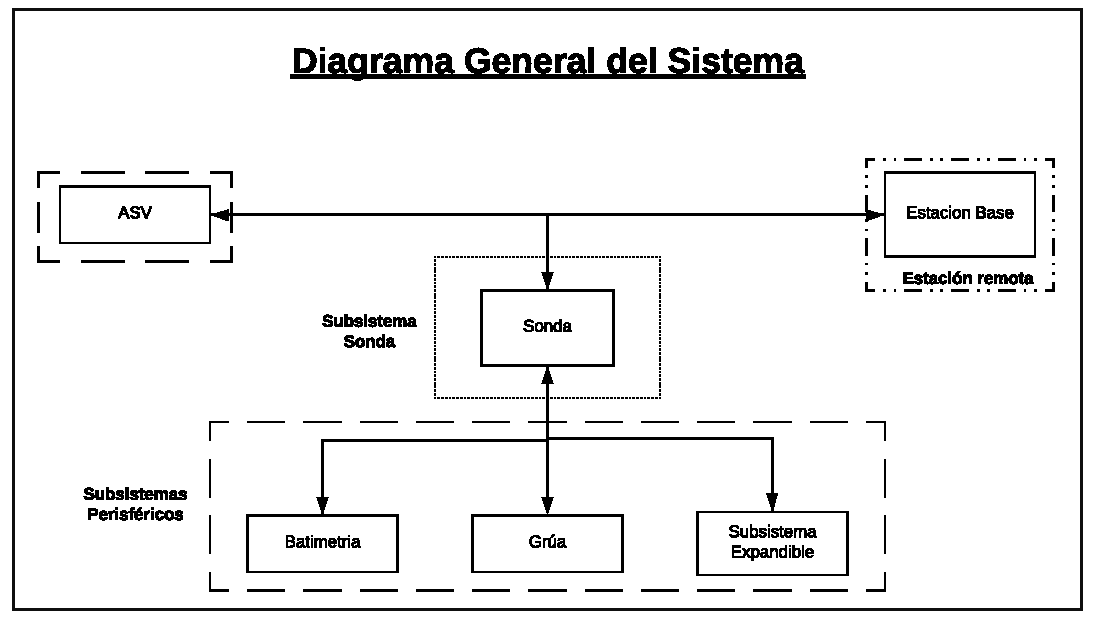
\includegraphics[width=150mm, height=70mm]{Imagenes/2021/img31.pdf}
    \caption[Diagrama General del Sistema]{Diagrama General del Sistema. \textbf{Fuente:} Elaboración Propia.}
    \label{fig:3.1}
\end{figure}

\subsubsection{Sonda}








\section{Aspectos Generales}
El desarrollo de la sonda implic\'o una serie de desaf\'ios t\'ecnicos, por ese motivo esa secci\'on se organiza de la siguiente manera

\begin{itemize}
    \item Dise\~no Mec\'anico: abarca todos los criterios considerados al dise\~no de la sonda y sistema de despliegue. 
    \item Fabricaci\'on Mec\'anica: abarca las t\'ecnicas y materiales empleadas para la fabricaci\'on de los componentes.
    \item Programaci\'on e Integraci\'on de los sensores: en esta secci\'on abarca lo referente a los distintos script desarrollados para lograr el funcionamiento del dispositivo.
\end{itemize}
\section{Dise\~no Mec\'anico}
Para el proceso de dise\~no se siguieron los procedimientos de XXX donde agrupan el proceso de dise\~no en las siguientes etapas:
Etapas del dise\~no: 

\subsection{Sonda}
\subsubsection{Conceptualizaci\'on}
Conceptualmente se definen los requerimientos m\'inimos para el correcto funcionamiento de la sonda.
\begin{itemize}
    \item versatilidad: su implementación debe de ser independiente a la dispositivo de soporte, pudiendo operar en cualquier medio de transporte.
    \item 
    \item Energ\'ia: la donde deber\'a tener autonom\'ia energ\'etica para sus operaciones de monitoreo,  
\end{itemize}
la donde deberá de contener en su interior al menos cinco sensores  (ph,CE,OD,OPR,T), adem\'as de toda la electr\'onica necesaria para la operaci\'on de estos. La sonda deber\'a tener autonom\'ia energ\'etica y poder sumergirse hasta una profundidad m\'inima de 5 metros , teniendo en cuenta que la profundidad promedio del lago Ypakarai es de 3 metros [\cite{hidrologiaItaipu}].
   
\subsubsection{An\'alisis}
En base a las conceptualizaci\'on de la secci\'on aterior y los materiales disponibles en el pa\'is se concluyen  :


\subsection{Despliegue}
\subsubsection{Conceptualizaci\'on}

deber\'a brindar soporte para que la sonda pueda hacer mediciones a varios niveles, dise\~no simple y adaptativo para ser instalado en embarcaciones de investigaci\'on.

\subsubsection{An\'alisis}
En base a las conceptualizaci\'on de la secci\'on aterior y los materiales dispobibles en el pa\'is se concluyen  :
\begin{itemize}
    \item Sonda: .
    \item Despliegue: deber\'a brindar soporte para que la sonda pueda hacer mediciones a varios niveles, dise\~no simple y adaptativo para ser instalado en embarcaciones de investigaci\'on.
\end{itemize}

\subsection{Diseño, Mecanizado de Piezas}



\section{Fabricaci\'on}





%-----------------------------------------------------------------------------




         

\subsection{Referencias Comerciales.}
Las pocas empresas que se dedican al rubro de la construcción de invernaderos Hidropónicos, las que se dedican al riego automatizado o las de ferti-riego ofrecen soluciones a proyectos de gran envergadura, debiéndose especificar siempre las hectáreas de plantación que se desean controlar para que tomen en cuenta el proyecto, lo diseñen y así puedan enviar un presupuesto al cliente interesado.
Según revisión de existencia local no existe un producto comercial del tipo de este trabajo dentro del territorio paraguayo.\textbf{}